\Question{Getting Started}

You may typeset your homework in latex or submit neatly handwritten and scanned solutions. Please make sure to start each question on a new page, as grading (with Gradescope) is much easier that way! Deliverables:

\begin{enumerate}
  \item Submit a PDF of your writeup to assignment on Gradescope, ``HW[n] Write-Up"
  \item Submit your test set evaluation results, ``HW[n] Test Set".
\end{enumerate}

After you've submitted your homework, be sure to watch out for the self-grade form.

\begin{Parts}

\Part Before you start your homework, write down your team. Who else did you work with on this homework? List names and email addresses. In case of course events, just describe the group. How did you work on this homework? Any comments about the homework?

\vspace{15pt}
\framebox(465, 75){}

\Part Please copy the following statement and sign next to it:

\textit{I certify that all solutions are entirely in my words and that I have not looked at another student's solutions. I have credited all external sources in this write up.}

\vspace{15pt}
\framebox(465, 75){}

\end{Parts}

\pagebreak
\Question{MLE of Multivariate Gaussian}

In lecture, we discussed uses of the multivariate Gaussian
distribution. We just assumed that we knew the parameters of the
distribution (the mean vector $\mu$ and covariance matrix
$\Sigma$). In practice, though, we will often want to estimate $\mu$
and $\Sigma$ from data. (This will come up even beyond regression-type
problems: for example, when we want to use Gaussian models for
classification problems.) This problem asks you to derive the Maximum
Likelihood Estimate for the mean and variance of a multivariate
Gaussian distribution. 

\begin{Parts}

% (a)
\Part Let $X$ have a multivariate Gaussian distribution with mean $\mu \in \mathbb{R}^d$ and covariance matrix $\Sigma \in \mathbb{R}^{d \times d}$. \textbf{Write the log likelihood of drawing the $n$ i.i.d. samples $x_1, \ldots, x_n \in \mathbb{R}^d$ from $X$ given $\Sigma$ and $\mu$}.



% (b)
\Part \textbf{Find MLE of $\mu$ and $\Sigma$.} For taking derivatives
with respect to matrices, you may use any formula in ``The Matrix
Cookbook'' without proof. This is a reasonably involved problem part
with lots of steps to get to the answer. We recommend students first
do the one-dimensional case and then the two-dimensional case to warm 
up. 



% (c)
\Part Use the following code to sample from a two-dimensional Multivariate Gaussian and plot the samples: 
\begin{verbatim}
	import numpy as np
	import matplotlib.pyplot as plt
	mu = [15, 5]
	sigma = [[20, 0], [0, 10]]
	samples = np.random.multivariate_normal(mu, sigma, size=100)
	plt.scatter(samples[:, 0], samples[:, 1])
	plt.show()
\end{verbatim}
Try the following three values of $\Sigma$:
$$\Sigma = [[20, 0], [0, 10]]; \Sigma = [[20, 14], [14, 10]]; \Sigma = [[20, -14], [-14, 10]].$$
\textbf{Calculate the mean and variance of these distributions from the samples (that is, implement part (b))}. Report your results. Include your code in your write-up.



\end{Parts}
\Question{Tikhonov Regularization and Weighted Least Squares}
In this problem, we view Tikhonov regularization from a probabilistic
standpoint. 

In lecture, you have seen this worked out in one way. In an earlier
homework, we introduced Tikhonov regularization as a generalization of
ridge regression. In this problem, you are mainly going to use the computer
to help deepen your understanding of how priors and thus the right
regularization can help. 

\begin{Parts}
\Part  Let $X \in \mathbb{R}^d$ be a $d$-dimensional random vector and
$Y \in \mathbb{R}$ be a one-dimensional random variable. Assume a
linear model between $X$ and $Y$: $Y=w^TX+z$ where $z\in\mathbb{R}$,
and $w\in\mathbb{R}^d$. Also assume that $z \sim N(0,1)$ is a Gaussian
random variable. Assume $w\sim N(0,\Sigma)$ where $\Sigma$ is a
symmetric positive definite matrix and this random variable is independent of the
observation noise. {\bf What is the conditional distribution of $Y$ given $X$ and $w$?}



\Part (Tikhonov regularization)  Given $n$ training data points
$\{(X_1,Y_1),(X_2,Y_2),\ldots, (X_n,Y_n)\}$ generated according to the
model of $(X,Y)$ in the previous part (the $w$ is common, but the
observation noise varies across the different training points. The $X_i$ are
distinct and are arbitrary.), {\bf derive the posterior distribution of $w$
given the training data.} Note: $w$ and $Y = (Y_1, Y_2, \ldots, Y_n)$ are jointly Gaussian in this
problem given the $X_i$. 

Hint: (You may or may not find this useful) If the probability density function of a random variable is of the form
\begin{equation} 
f(X)=C \cdot\exp\{-\frac{1}{2}X^TAX+b^TX\}, 
\end{equation}
where $C$ is some constant to make $f(X)$ integrates to $1$, then the mean of $X$ is 
$A^{-1}b$. This can be used to help complete squares if you choose to
go that way.

This case was derived in lecture, and you are free to replicate the
derivation from lecture in your own language. You are also free to
give a different derivation from first principles if you like.



\Part {\bf (BONUS but in-scope.)} How would you extend your result from
the previous part to the case where the observation noise $Z$ was no
longer $N(0, 1)$ but was instead distributed as $N(\mu_z, \Sigma_z)$ for
some mean $\mu_z$ and some covariance $\Sigma_z$, but was independent
of the parameter $w$. {\bf Give an argument based on appropriately
  changing coordinates.}


\Part (Compare the effect of different priors) Do the following for
$\Sigma = \Sigma_1,\Sigma_2,\Sigma_3,\Sigma_4,\Sigma_5,\Sigma_6$ respectively, where 
\begin{align*}
\Sigma_1 &= \begin{bmatrix}
    1      & 0\\
    0      & 1
    \end{bmatrix} \\
\Sigma_2 &= \begin{bmatrix}
1      & 0.25\\
0.25      & 1
\end{bmatrix} \\
\Sigma_3 &= \begin{bmatrix}
1      & 0.9\\
0.9      & 1
\end{bmatrix} \\
\Sigma_4 &= \begin{bmatrix}
1      & -0.25\\
-0.25      & 1 
\end{bmatrix}  \\
\Sigma_5 &= \begin{bmatrix}
1      & -0.9\\
-0.9      & 1 
\end{bmatrix}  \\
\Sigma_6 &= \begin{bmatrix}
0.1      & 0 \\
0      & 0.1 
\end{bmatrix}  
\end{align*} 
In the above cases, the priors on the two parameters are independent
with large variance, mildly positively correlated, strongly positively
correlated, mildly negatively correlated, strongly negatively
correlated, and then independent with small variances respectively. 

Generate $5, 50,$ and $500$ data points from $Y=X_1+X_2+Z$ where
$X_1,X_2 \sim N(0,5)$ and $Z\sim N(0,1)$ as training data. {\bf Plot the contours of the posteriors on
  $w$ for all 18 cases of assumed priors and number of data points. What do you observe?}

Hint: Use matplotlib.mlab.bivariate\_normal to generate the value of pdf for bivariate normals.  


\Part (Influence of Priors) Generate $n$ training data samples from
$Y=X_1+X_2+Z$ where $X_1,X_2 \sim N(0,5)$ and $Z\sim N(0,1)$ as
before. Notice that the true parameters $w_1 = 1, w_2 = 1$ are
moderately large and positively correlated with each other. We want to
quantitatively understand how the effect of the prior influences the
mean square error as we get more training data.  This should
corroborate the qualitative results you saw in the previous part.

In this case, we could directly compute the ``test error'' once we see
the estimated parameters. Namely, if we estimate after learning that
the model is $Y = \widehat{w}_1 X_1 + \widehat{w}_2 X_2 + Z$, the
average test error should theoretically be $5(\widehat{w}_1-1)^2 +5(\widehat{w}_2 -
1)^2 + 1$. (Make sure you understand why.)

However, it is good to also keep in mind what happens with a finite
amount of test data. So, generate a test set of $100$ data points
from this model and use the test error on that to evaluate what
happens as we use more training data. 

If we just plotted the average test-error (or the theoretical average
test error) with respect to the amount of training data, we still have
the randomness in the specific training data that was
used. Consequently, it is worth replicating this experiment a few
times (say 20 times) to get an average of averages. (It is also
insightful to look at the spread.) 

{\bf Plot the mean square error between $\hat Y_i$ and $Y_i$ over the
  test data with respect to the size of training data $n$ (increase
  $n$ from $5$ to $200$ by $5$). Include what the theoretical mean
  square error should be for those parameter estimates. Compare what
  happens for different priors as the amount of training data increases.}

Recall the MSE is defined by
\begin{equation}
\frac{1}{n}\sum_{i=1}^n(Y_i-\hat{Y}_i)^2. 
\end{equation}

Here $\hat{Y}_i = \widehat{w}^TX_i$ where $X_i\in\mathbb{R}^2$ and
$\widehat{w}$ in your model is the solution to the least square
problem with Tikhonov regularization given the training data.   

You should observe that
\begin{itemize}
    \item Enough data will wash away the effects of the prior.
    \item A good prior helps when there are not enough data points.
\end{itemize}
\end{Parts}
\Question{Total Least Squares}

Recall that in the least squares problem, we want to solve for $\vec{w}$ in $\min_{\vec{w}}{||A\vec{w}-\vec{y}||}$. We measure the error as the difference between $A\vec{w}$ and $\vec{y}$, which can be viewed as adding an error term $\hat{\vec{y}}$ such that the equation $A\vec{w}=\vec{y}+\hat{\vec{y}}$ has a solution:

\begin{align}
\min\lvert\lvert\hat{\vec{y}}\rvert\rvert_F,\text{ subject to }A\vec{w}=\vec{y}+\hat{\vec{y}}
\label{eq:ls_min}
\end{align}

Although this optimization formulation allows for errors in the measurements of $\vec{y}$, it does not allow for errors in the feature matrix $A$ that is measured from the data.  In this problem, we will explore a method called \emph{total least squares} that allows for both error in the matrix $A$ and the vector $\vec{y}$, represented by $\hat{A}$ and $\hat{\vec{y}}$, respectively.  Specifically, the total least squares problem is to find the solution for $\vec{w}$ in the following minimization problem:

\begin{align}
\min\lvert\lvert[\hat{A},\hat{\vec{y}}]\rvert\rvert_F,\text{ subject to }(A+\hat{A})\vec{w}=\vec{y}+\hat{\vec{y}}
\label{eq:tls_min}
\end{align}

where the matrix $[\hat{A},\hat{y}]$ is the concatenation of the columns of $\hat{A}$ with the column vector $\vec{y}$.  Intuitively, this equation is finding the smallest perturbation to the matrix of data points $A$ and the outputs $\vec{y}$ such that the linear model can be solved exactly. This minimization problem can be rewritten as

\begin{align}
\min_{\hat{A},\hat{\vec{y}}}[A+\hat{A},\vec{y}+\hat{\vec{y}}]\begin{bmatrix}\vec{w}\\-1\end{bmatrix}=\vec{0}
\label{eq:tls}
\end{align}

\begin{Parts}

\Part Let the matrix $A\in\mathbb{R}^{n\times d}$ and $\vec{y}\in\mathbb{R}^n$.  Assuming that $n>d$ and $\text{rank}(A+\hat{A})=d$, \textbf{explain why $\text{rank}([A+\hat{A},\vec{y}+\hat{\vec{y}}])=d$.}



\Part We know that the matrix $[A+\hat{A},\vec{y}+\hat{\vec{y}}]$ is degenerate (has less than full rank).  Therefore, by the Eckart-Young-Mirsky Theorem which tells us what the closest lower-rank matrix in the Frobenius norm is, the matrix $[A+\hat{A},\vec{y}+\hat{\vec{y}}]$ that minimizes the problem is given by

\begin{align*}
[A,\vec{y}]&=U\Sigma V^\top\\
[A+\hat{A},\vec{y}+\hat{\vec{y}}]&=U
\begin{bmatrix}
\Sigma_{1,...,d}&\\&0
\end{bmatrix}
V^\top
\end{align*}

where $\Sigma_{1,..,d}$ is the diagonal matrix of the $d$ largest singular values of $[A,\vec{y}]$.  \textbf{Using this information, find a nonzero solution to $[A+\hat{A},\vec{y}+\hat{\vec{y}}]\vec{x}=\vec{0}$ and thus solve for $\vec{w}$ in Equation~\ref{eq:tls}.}

\emph{HINT: the last column of the product $[A,\vec{y}]V$ will be useful}



\Part In this problem, we will use total least squares to approximately learn the lighting in a photograph, which we can then use to paste new objects into the image while still maintaining the realism of the image.  You will be estimating the lighting coefficients for the interior of St.~Peter's Basillica, and you will then use these coefficients to change the lighting of an image of a tennis ball so that it can be pasted into the image.  In Figure~\ref{fig:noshade}, we show the result of pasting the tennis ball in the image without adjusting the lighting on the ball.  The ball looks too bright for the scene and does not look like it would fit in with other objects in the image.

\begin{figure}
\centering
  \begin{minipage}[b]{0.4\textwidth}
  \includegraphics[width=\textwidth]{src/problems/least_squares/tennis_no_shade}
  \end{minipage}
    \begin{minipage}[b]{0.4\textwidth}
  \includegraphics[width=\textwidth]{src/problems/least_squares/tennis_lsq}
  \end{minipage}

\caption{Tennis ball pasted on top of image of St.~Peter's Basillica without lighting adjustment (left) and with lighting adjustment (right)
}\label{fig:noshade}
\end{figure}

To start, we will represent environment lighting as a spherical function $\vec{f}(\vec{n})$ where $\vec{n}$ is a 3 dimensional unit vector ($\lvert\lvert\vec{n}\rvert\rvert_2=1$), and $\vec{f}$ outputs a 3 dimensional color vector, one component for red, green, and blue light intensities.  Because $\vec{f}(\vec{n})$ is a spherical function, the input must correspond to a point on a sphere. In this case, we are using normalized vectors in 3 dimensions to represent a point on a sphere.  The function $\vec{f}(\vec{n})$ represents the total incoming light from the direction $\vec{n}$ in the scene.

To convincingly add an object to an image, we need to need to apply the lighting from the environment onto the added object.  In this case, we'll be adding a tennis ball to the scene.  Because the tennis ball is what's considered a diffuse surface, the color of a point on the ball can be computed as a weighted sum of all of the incoming light at that point that has a positive dot product with the direction $\vec{n}$.  This weighted sum can be approximated by blurring the image used to estimate the lighting environment.  However, we skip this blurring step and instead approximate the spherical function $\vec{f}(\vec{n})$ in terms of the first 9 spherical harmonic basis functions, where spherical harmonics are like the Fourier transform but for spherical functions.  Because we are using only 9 of the basis functions, most of the information in the image cannot be captured, which will effectively blur the image.

\begin{figure}
\centering
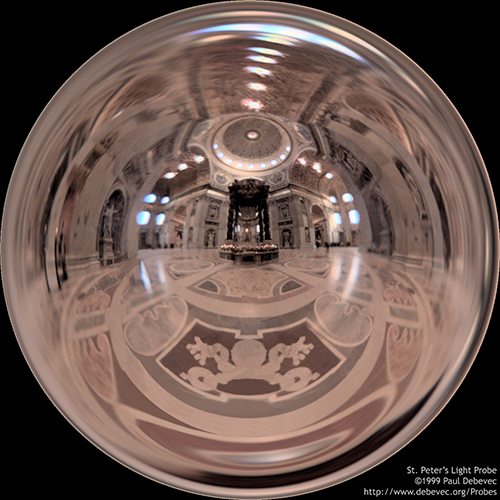
\includegraphics[width=0.4\textwidth]{src/problems/least_squares/stpeters_probe_small}
\caption{Image of a spherical mirror inside of St. Peter's Basillica}
\label{fig:probe}
\end{figure}

The first 9 unormalized basis functions are given by:

\begin{align*}
L_{0,0}&=1\\
L_{1,-1}&=y\\
L_{1,1}&=x\\
L_{1,0}&=z\\
L_{2,-2}&=x*y\\
L_{2,-1}&=y*z\\
L_{2,0}&=3*z^2-1\\
L_{2,1}&=x*z\\
L_{2,2}&=x^2-y^2
\end{align*}

where $\vec{n}=[x,y,z]^\top$.  The lighting function can then be approximated as

\begin{align*}
\vec{f}(\vec{n})\approx\sum_{i=1}^9 \vec{\gamma}_i L_i(\vec{n})
\end{align*}

where $L_i(\vec{n})$ is the $i$th basis function from the list above.

The function of incoming light $\vec{f}(\vec{n})$ can be measured by photographing a spherical mirror placed in the scene of interest.  In this case, we provide you with an image of the sphere as seen in Figure~\ref{fig:probe}.  In the code provided, there is a function extractNormals(img) that will extract the training pairs $(\vec{n}_i,\vec{f}(\vec{n}_i))$ from the image.  An example using this function is in the code.

\textbf{Use the spherical harmonic basis functions to create a $9$ dimensional feature vector for each sample.  Use this to formulate an ordinary least squares problem and solve for the unknown coefficients $\vec{\gamma}_i$.  Report the estimated values for $\vec{\gamma}_i$ and include a visualization of the approximation using the provided code.} The code provided will load the images, extracts the training data, relights the tennis ball with incorrect coefficients, and saves the results.  Your task is to compute the basis functions and solve the least squares problems to provide the code with the correct coefficients.  To run the starter code, you will need to use Python with \texttt{numpy} and \texttt{scipy}.  Because the resulting data set is large, we reduce it in the code by taking every $50^\text{th}$ entry in the data.  This is done for you in the starter code, but you can try using the entire data set or reduce it by a different amount.



\Part When we estimate the direction $\vec{n}$ to compute our training data  $(\vec{n}_i,\vec{f}(\vec{n}_i))$, we make some approximations about how the light is captured on the image.  We also assume that the spherical mirror is a perfect sphere, but in reality, there will always be small imperfections.  Thus, our measurement for $\vec{n}$ contains some error, which makes this an ideal problem to apply total least squares.  \textbf{Solve this problem with total least squares by allowing perturbations in the matrix of basis functions.  Report the estimated values for $\vec{\gamma}_i$ and include a visualization of the approximation.}  The output image will be visibly wrong, and we'll explore how to fix this problem in the next part.  Your implementation may only use the SVD and the matrix inverse functions from the linear algebra library in numpy.



\Part In the previous part, you should have noticed that the visualization is drastically different than the one generated using least squares.  This difference is caused by the difference in scale between the inputs and the outputs.  The inputs are all unit vectors, and the outputs are 3 dimensional vectors where each value is in $[0,384]$.  Typically, values in an image will be in $[0,255]$, but the original image had a much larger range.  We compressed the range to a smaller scale using tone mapping, but the effect of the compression is that relatively bright areas of the image become less bright.  As a compromise, we scaled the image colors down to a maximum color value of $384$ instead of $255$. \textbf{Explain why the difference in the range of values for the inputs $L_i(\vec{n})$ and the outputs $\vec{f}(\vec{n}_i)$ would create this difference in results when solving the total least squares problem.  Propose a value by which to scale the outputs $\vec{f}(\vec{n}_i)$ such that the values of the inputs and outputs are roughly on the same scale. Solve this scaled total least squares problem, report the computed spherical harmonic coefficients and provide a rendering of the relit sphere.}



\end{Parts}

\pagebreak

\Question{Your Own Question}

{\bf Write your own question, and provide a thorough solution.}

Writing your own problems is a very important way to really learn
material. The famous ``Bloom's Taxonomy'' that lists the levels of
learning is: Remember, Understand, Apply, Analyze, Evaluate, and
Create. Using what you know to create is the top-level. We rarely ask
you any HW questions about the lowest level of straight-up
remembering, expecting you to be able to do that yourself. (e.g. make
yourself flashcards) But we don't want the same to be true about the
highest level.

As a practical matter, having some practice at trying to create
problems helps you study for exams much better than simply counting on
solving existing practice problems. This is because thinking about how
to create an interesting problem forces you to really look at the
material from the perspective of those who are going to create the
exams. 

Besides, this is fun. If you want to make a boring problem, go
ahead. That is your prerogative. But it is more fun to really engage
with the material, discover something interesting, and then come up
with a problem that walks others down a journey that lets them share
your discovery. You don't have to achieve this every week. But unless
you try every week, it probably won't happen ever. 